\section{Background and Literature Review}\label{sec:literature}

Offshore wind is usually measured in gigawatts installed and terawatt-hours
generated. Neither quantity determines whether a wind farm earns money. A
generator is paid the price prevailing in the hours it produces, and because
wind output across a sea basin arrives together, those are precisely the hours
in which the price is lowest. This chapter builds the argument from that single
observation. Section~\ref{sec:markets} sets out how European wholesale prices
form. Section~\ref{sec:value_problem} defines the resulting value erosion and
reviews its measured magnitude. Section~\ref{sec:mitigation} asks the question
on which this thesis turns, namely whether that erosion is an inherent property
of the resource or a consequence of system design that can be reversed.
Section~\ref{sec:two_seas} contrasts the two basins under study, and
Section~\ref{sec:modelling} reviews the model families available for
answering the question. Section~\ref{sec:research_gap} states the gaps that
remain and the questions this thesis puts to them.

\subsection{Price formation in electricity markets}\label{sec:markets}

The day-ahead market, which carries 80 to 90\,\% of merchant wind revenue
\cite{Jansen2020}, clears pay-as-clear. Generators offer at short-run
marginal cost, the market operator stacks those offers into an ascending supply
curve, and every dispatched unit receives the price of the most expensive unit
required to meet demand. Wind turbines, whose fuel is free, enter at the bottom
of that stack. Additional wind shifts the supply curve to the right,
displaces the marginal thermal unit, and lowers the clearing price. This is the
merit order effect, illustrated in Figure~\ref{fig:merit_order}.

\begin{figure}[!htb]
    \centering
    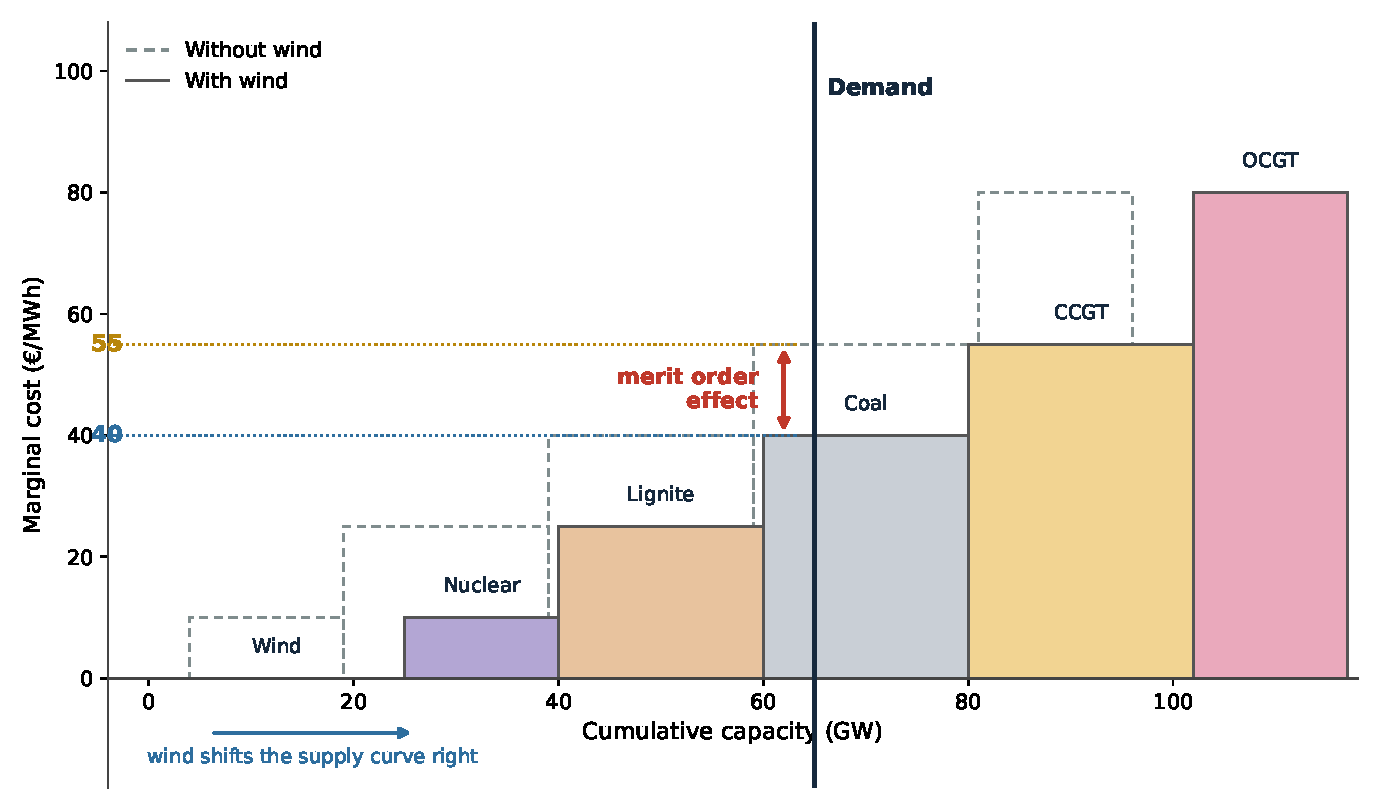
\includegraphics[width=0.82\textwidth]{merit_order_effect}
    \caption{The merit order effect. Wind enters at the bottom of the supply
    curve and shifts it rightward, displacing higher-cost thermal plant and
    reducing the clearing price from 55 to 40~\euro/MWh in this stylised
    example. The depression is deepest in exactly the hours wind generates
    most.}
    \label{fig:merit_order}
\end{figure}

Prices are not formed zone by zone in isolation: the Single Day-Ahead Coupling
mechanism matches orders across participating zones simultaneously, subject to
available cross-zonal transmission \cite{EUPHEMIA2020}. Where transmission is
adequate prices converge and the merit order effect is shared across borders;
where it binds, prices separate and the surplus is trapped \cite{Newbery2018}.
A basin cannot be analysed as a closed system.

Geographic resolution matters as much as mechanism. Europe is divided into
bidding zones, each clearing at one price: Germany prices a single zone despite
substantial internal congestion, a configuration under review whose resolution
would change North Sea wind revenues \cite{Egerer2015, GermanBZSplit2024}, while
the Nordic countries split into eleven zones that let transmission constraints
surface as genuine price areas \cite{Fridolfsson2009}. The three Baltic states
each form their own zone and, since February 2025, are synchronised with the
continental grid rather than the former Soviet system
\cite{BalticSynchronisation2025, ACER2025}.
Figure~\ref{fig:bidding_zones} sets out the zones around both basins with the
interconnectors between them, and groups them by the kind of generation that
usually sets their price, which is the distinction Section~\ref{sec:two_seas}
develops. A zonal structure localises price signals, so cannibalisation
propagates to neighbours only as far as interconnection carries it.

\begin{figure}[!htb]
    \centering
    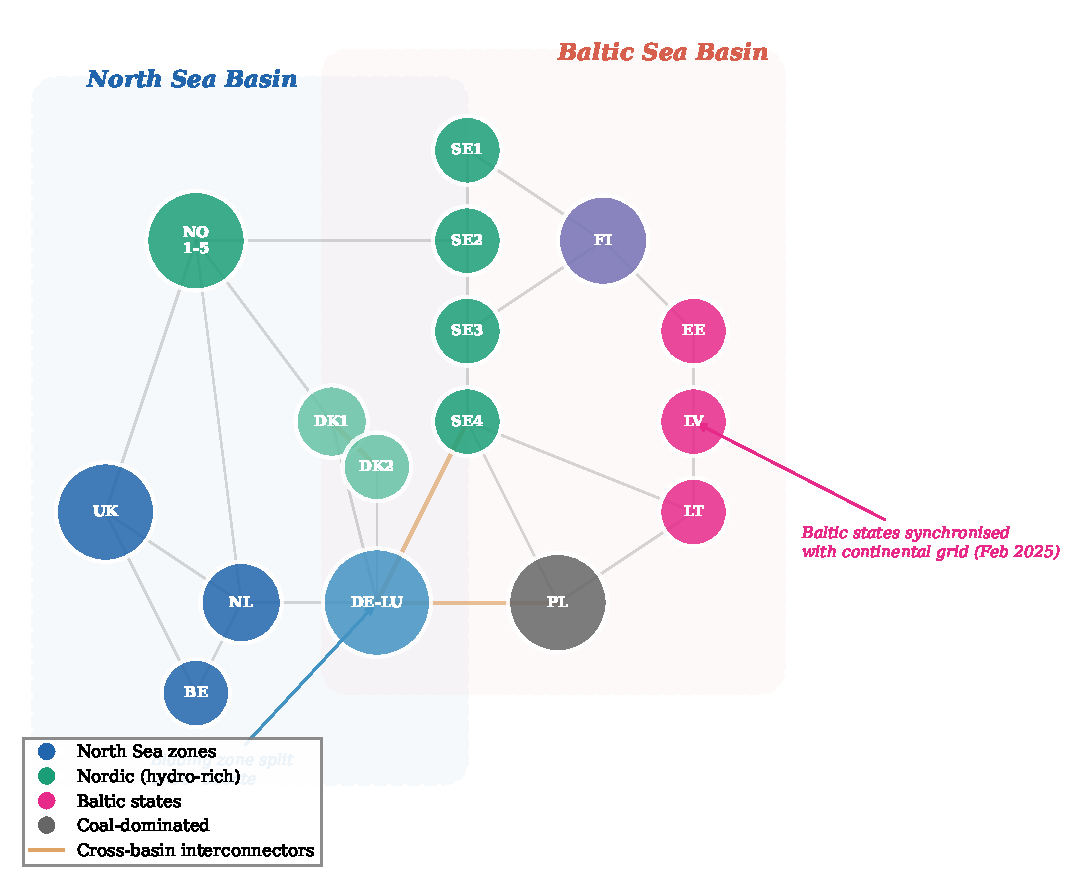
\includegraphics[width=0.78\textwidth]{bidding_zones_map}
    \caption{Bidding zones and the main interconnectors around the North Sea
    and the Baltic. Zones are grouped by the kind of generation that usually
    sets their price: North Sea markets, hydro-rich Nordic markets, the Baltic
    states, which synchronised with the continental grid in February 2025, and
    coal-dominated systems. Interconnectors between the two basins are drawn in
    orange.}
    \label{fig:bidding_zones}
\end{figure}

\subsection{Capture price, cannibalisation and value erosion}\label{sec:value_problem}

\subsubsection{Capture price and capture value}

A baseload plant running continuously earns approximately the time-averaged
wholesale price; a wind farm earns the average price weighted by its own output.
Two measures established by Hirth \cite{Hirth2013} formalise the difference. The
\textit{capture price} is the generation-weighted average spot price received.
Dividing it by the baseload price, the simple time-average of the wholesale
price over the same period, gives the \textit{capture value}:
%
\begin{equation}
    \text{Capture value} = \frac{\text{Capture price}}{\text{Baseload price}}
    = \frac{\sum_{t} p_t \, g_t}{\bar{p} \sum_{t} g_t}
    \label{eq:value_factor}
\end{equation}
%
where $p_t$ is the spot price in hour $t$, $g_t$ the generation, and $\bar{p}$
the time-averaged price. At negligible penetration the ratio sits near unity; as
wind's share grows its own output moves the price in the hours it generates and
the ratio falls. That shortfall is what Hirth \cite{Hirth2015} and Ueckerdt et
al. \cite{Ueckerdt2013} term profile cost, and it is precisely the quantity a
cost-only assessment of where to build omits.

Hirth's early estimates placed the decline at roughly 1.10 at negligible
penetration falling to between 0.50 and 0.80 at a 30\% wind share, the range
separating thermal-dominated systems from hydro-dominated ones
(Figure~\ref{fig:capture_value_decline}) \cite{Hirth2013}. That spread is not
incidental here: most North Sea markets are thermal-heavy, the Baltic rim
borders Scandinavian hydro. Later work at higher penetration has confirmed the
pattern and established that the decline steepens as penetration rises
\cite{Stiewe2025, LopezProl2024, Ember2025, Cevik2022}.

\begin{figure}[!htb]
    \centering
    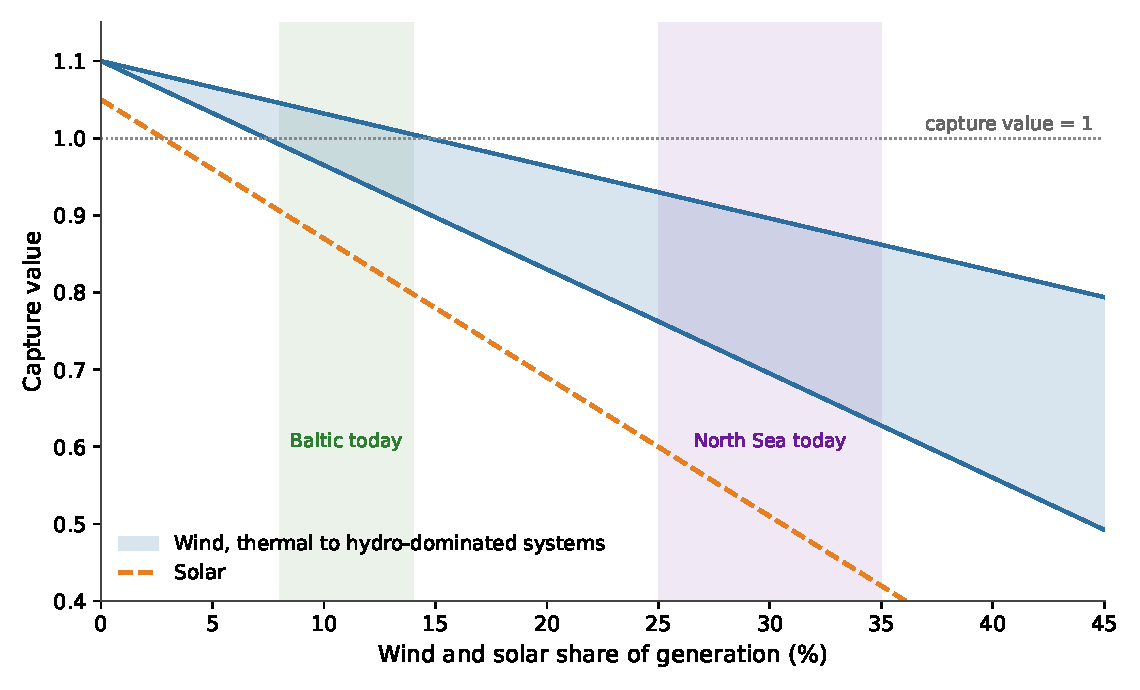
\includegraphics[width=0.7\textwidth]{capture_value_decline}
    \caption[Capture value against wind and solar market share]{Capture value against wind and solar market share,
    synthesised from Hirth \cite{Hirth2013}. The shaded band for wind spans
    thermal-dominated systems (lower bound) to hydro-dominated systems (upper
    bound); the approximate current penetration ranges of the North Sea and
    Baltic markets are indicated.}
    \label{fig:capture_value_decline}
\end{figure}

Figure~\ref{fig:capture_value_traj} shows the divergence directly. Germany's
capture value fell from 0.93 to 0.76 as wind penetration rose from roughly 20\%
to 35\%, while Poland, where wind remained below 18\% of generation and coal
sets the marginal price in most hours, stayed near unity. The Scandinavian
markets sit between the two, buffered by hydro, and the 2021 to 2022 uptick is
the gas crisis lifting wholesale prices faster than capture prices could follow.
The spread between the highest and lowest trajectories widened from five
percentage points in 2015 to twenty by 2024, which is both the severity of the
problem and the reason a basin-level comparison is worth making.

\begin{figure}[!htb]
    \centering
    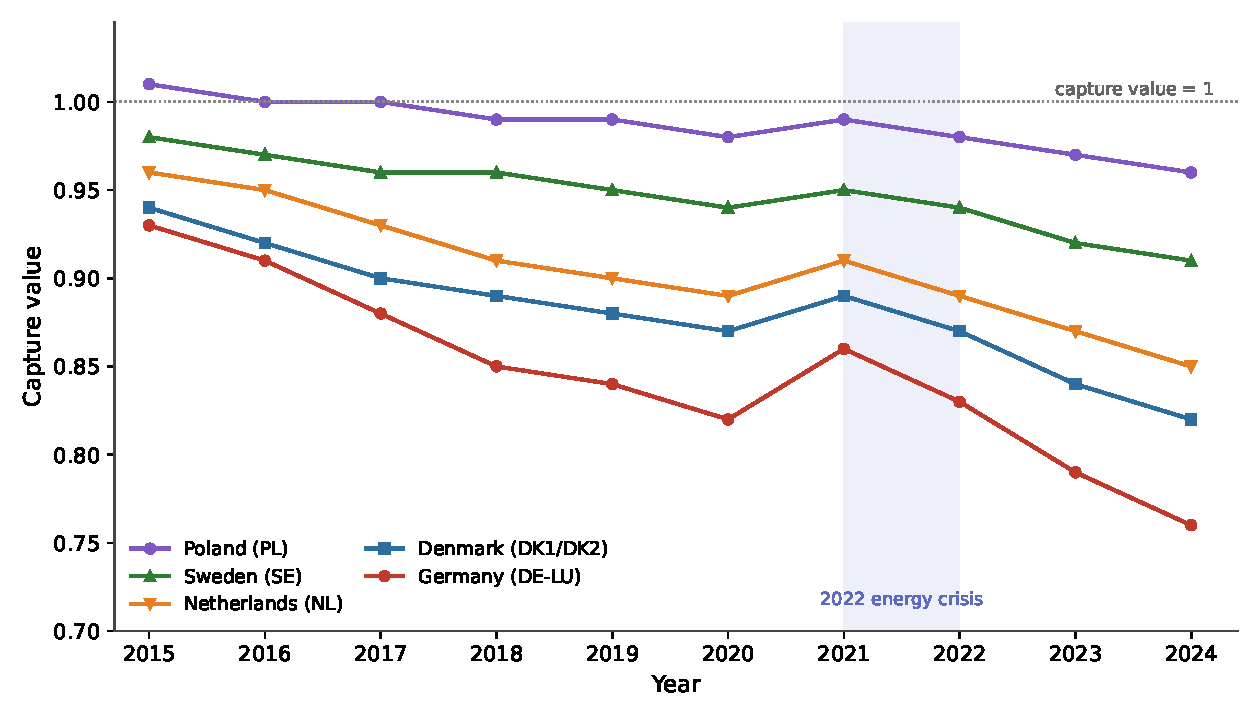
\includegraphics[width=0.86\textwidth]{capture_value_trajectories}
    \caption[Observed offshore capture value, 2015 to 2024]{Observed wind
    capture value for selected European bidding zones, 2015 to 2024, computed as
    the ratio of generation-weighted capture price to baseload price.
    Synthesised from Stiewe et al. \cite{Stiewe2025}, Ember
    \cite{Ember2025, EmberGlobal2024} and ACER market monitoring
    \cite{ACER2023, ACER2025}. The 2021 to 2022 uptick reflects the temporary
    elevation of wholesale prices during the gas crisis.}
    \label{fig:capture_value_traj}
\end{figure}

\subsubsection{Magnitude and measurement}

Estimates of the merit order effect span more than an order of magnitude across
markets, periods and methods \cite{Sensfuss2008, Cludius2014, Lunackova2017},
partly genuine variation and partly the fragility of the identification
assumptions behind them \cite{Wurzburg2013, Clo2015, Kolb2020}. For Baltic
markets published estimates are effectively absent, the pan-European panel of
Cevik and Ninomiya \cite{Cevik2022} being the only work that includes Baltic
zones, and that absence is part of the motivation for this thesis.

Cevik and Ninomiya find that each percentage point of additional renewable share
reduces average wholesale prices by 0.6\%, accelerating at higher penetration
\cite{Cevik2022}. Since wind sells precisely in the hours its own output has
depressed \cite{Hirth2013}, erosion becomes severe past roughly a 20\% wind
share, beyond which Hirth estimates additional wind stops adding system welfare
\cite{HirthOptimal2015}. Offshore is more exposed than onshore: higher and
steadier capacity factors concentrate output in time and correlate it across a
basin, so a sustained blow depresses prices across several coupled zones at once
\cite{Yamujala2026}.

\subsubsection{From price depression to cannibalisation}

The merit order effect describes an instantaneous price depression;
cannibalisation is its cumulative consequence, the revenue earned per
megawatt-hour falling for every existing and prospective asset as capacity
accumulates. Its severity depends on penetration, the spatial correlation of
output, fuel and carbon prices, and the flexibility of the surrounding system
\cite{Hirth2013, Stiewe2025}. Its most visible symptom is the growth of negative
prices, abundant wind meeting inflexible plant that will not curtail and
generators that keep producing because support rewards volume; negative hours
have risen sharply where penetration is highest
\cite{Ember2025, EmberGlobal2024}, masked briefly by the 2022 crisis and
reasserted as gas normalised \cite{Ruhnau2023}. The German fall of
Figure~\ref{fig:capture_value_traj} compounds higher penetration, greater temporal
concentration of offshore output, and the inflexibility of lignite
\cite{Monteil2023, Stiewe2025, Ember2025}.

Whether this is permanent is contested: theory predicts convergence as marginal
generators exit \cite{Antweiler2021, Brown2021}, but European support decouples
investment from market signals and delays that exit \cite{Hirth2013}. The gap is
starkest in small, fast-expanding Baltic markets, where projected revenue losses
reach 15 to 20~\euro/MWh by 2029 against near-zero today
\cite{BalticCannibalisation2024_studies}, too fast for the fleet adjustments
equilibrium arguments assume.

\subsubsection{Cross-border cannibalisation effects}

Most analyses treat each bidding zone as an island. Stiewe et al.
\cite{Stiewe2025} tested that directly, regressing the domestic capture value on
both domestic wind penetration and that of directly interconnected neighbours
across more than 30 zones from 2015 to 2023. A one point rise in domestic
penetration removes 0.61 points of capture value; a simultaneous one point rise
across all neighbours removes a further 0.33, so coordinated European expansion
costs nearly a full point for every point added. The profitability of a Danish
wind farm depends on Dutch, German, Norwegian and Swedish deployment as well as
Danish.

Two features of that identification, the fixed effects absorbing each market's
character and the linear penetration term, are structural limits of statistical
models, and Section~\ref{sec:modelling} returns to what they imply for
projection.

\subsection{Moderators of cannibalisation}\label{sec:mitigation}

The literature so far establishes that capture value falls with penetration
and that the fall propagates across borders, but it largely treats the
surrounding system as fixed. Every mechanism above depends on system
configuration: whether surplus can leave the zone, whether anything absorbs
it, where the fleet is placed, and who is contractually exposed. This section
reviews those four levers.

\subsubsection{Interconnection}

Transmission plays a dual role: capacity exports surplus, relieving domestic
price depression, but imports the depression of high wind next door. Stiewe
et al. find the mitigating effect slightly outweighs the exacerbating one
\cite{Stiewe2025}, and at system scale the benefit is larger, transmission
expansion cutting the total cost of a highly renewable European grid by
roughly 25\% \cite{Schlachtberger2017}.

The scale of planned investment reflects this: more than \euro{}400~billion
of offshore transmission by 2050 under the ENTSO-E Offshore Network
Development Plan \cite{ONDP2024}, with the 70\% cross-zonal trading
requirement pushing markets toward convergence \cite{ACER2023, ACER2025}.
Convergence is double-edged for a generator: surplus exports more easily,
while the importing zone absorbs the corresponding depression.

Congestion is also a revenue stream: whenever a link binds the price differs
across it, and the rent accrues to transmission operators. Joskow and Tirole
\cite{JoskowTirole2005} formalised the awkward consequence, that an investor
relieving the constraint destroys the income justifying the investment, which is
why regulated planning dominates. Article~19 of Regulation (EU) 2019/943
ring-fences those revenues for maintaining or increasing cross-zonal capacity
\cite{EURegulation2019943}, so a congested basin is already earmarking the money
that would relieve it. Neither that accounting nor the question of how much of a
zone's capture value decline is transmission scarcity rather than penetration
has been brought together with capture value analysis, and this thesis
undertakes the decomposition.

\subsubsection{Flexibility and sector coupling}

Storage and conversion attack the same problem in time rather than space.
Hybrid configurations pairing offshore wind with electrolysis absorb surplus
locally \cite{OffshoreHybrids2024}, sector coupling converts it into demand that
would not otherwise exist \cite{Brown2021}, and demand-side flexibility remains
largely unquantified \cite{Hirth2015}. The important observation is negative:
none of these pathways has been integrated into spatial capture value
assessment, so published projections implicitly assume that today's level of
flexibility persists into the future, an assumption that has not been tested at
the scale of a whole basin.

\subsubsection{Spreading the fleet}

The third lever is spatial: if output arrives everywhere at once, placing
capacity where it blows at different times should raise the portfolio's value.
The idea is Markowitz's mean-variance argument \cite{Markowitz1952} applied to
European wind by Roques et al. \cite{Roques2010}. Two things follow that the
literature has not pursued: portfolio treatments optimise the variance of
\textit{generation} while an investor is exposed to the variance of
\textit{revenue}, which market coupling can correlate even where wind is not;
and the mean effect has been neglected, since less severe cannibalisation
arrives as higher average capture value rather than lower volatility.

\subsubsection{Support mechanisms and risk allocation}

The fourth lever is contractual, and it determines not whether value is lost but
who loses it. European governments have moved from guaranteed feed-in tariffs
toward instruments that expose generators to price risk while structuring how it
is shared (Table~\ref{tab:support_mechanisms}).

\begin{table}[!htb]
\centering
\small
\caption{Principal revenue support mechanisms for offshore wind. Market exposure
ranges from none, under a fixed feed-in tariff, to full, under merchant
operation. Two-sided contracts for difference dominate North Sea procurement,
while certificate and premium schemes remain more common around the Baltic.
Basin prevalence is as of 2024.}
\label{tab:support_mechanisms}
\resizebox{\textwidth}{!}{%
\begin{tabular}{l p{7cm} l l}
\toprule
\textbf{Mechanism} & \textbf{Description} & \textbf{Market exposure} & \textbf{Basin prevalence} \\
\midrule
Feed-in tariff & Fixed payment per MWh, independent of market price & None & Legacy, phased out \\
\addlinespace
Two-sided CfD & Strike price agreed; the state pays any shortfall and the generator returns any surplus & Medium & North Sea (UK, NL, DE, PL) \\
\addlinespace
Electricity certificates & Tradable credits per MWh, valued by a separate certificate market & High & Baltic (SE) \\
\addlinespace
Premium schemes & Fixed or sliding premium added to the wholesale price & Medium to high & Baltic states (LT, LV, EE) \\
\addlinespace
Merchant & No direct support; revenue follows wholesale prices entirely & Full & Emerging (NL, DE) \\
\bottomrule
\end{tabular}%
}
\end{table}

The two-sided contract for difference has become dominant: the state pays the
difference when the wholesale price falls below the strike and recovers it
above. The stabilisation lengthens debt tenors and lowers risk margins
\cite{Beiter2024, Dukan2025}, an effect Kitzing et al. argue is structural,
since without it the cost of capital rises enough to negate a decade of
levelised-cost reductions \cite{Kitzing2024}. Premium and certificate schemes
leave operators exposed in exactly the hours cannibalisation is most severe
\cite{Dukan2025}, and the 2024 EU market reform mandated two-sided contracts for
all new supported capacity \cite{EUMarketReform2024}. The geography differs: the
North Sea has converged on mature contract-for-difference frameworks
\cite{WindEurope2025} while the Baltic rim remains a patchwork
\cite{Anatolitis2025}. What this literature does not do is connect contract
design back to the physical decomposition, asking which component of a capture
value decline a given instrument absorbs. That question is taken up here.

\subsection{The North Sea and Baltic Sea as contrasting market environments}\label{sec:two_seas}

\subsubsection{Wind resource and correlation}

European wind is governed by the westerly circulation carrying Atlantic systems
eastward, modulated by weather regimes that swing European mean wind generation
by a factor of two \cite{Grams2017}. Both basins respond to the same patterns,
but partial shielding by the Scandinavian land mass gives the Baltic some
decorrelation from the North Sea.

The resource is unambiguously stronger in the west: mean speeds near
9.75~m\,s$^{-1}$ against 7.5 to 8.0 \cite{Karagali2013}, capacity factors of 40
to 50\% against 35 to 40\% \cite{Solbrekke2022}. The gap narrows once wake
losses are counted, German Bight clusters losing wind speed for up to 70~km
downstream \cite{Schneemann2022} where the sparser Baltic is less affected.

Correlation structure matters as much as resource strength, because simultaneous
output depresses the same hours. Wind power correlation decays exponentially
with distance \cite{Louie2014, Olauson2016} but neither isotropically nor
uniformly: east-west pairs lag as Atlantic fronts propagate eastward, so a North
Sea event precedes its Baltic counterpart by several hours \cite{Malvaldi2017},
and cross-basin correlations sit consistently below within-basin ones
\cite{Olauson2016}. Mehrens et al. \cite{Mehrens2016} estimate a decorrelation
length of about 425~km (Figure~\ref{fig:correlation_decay}); set against the
North Sea's span of roughly 580 by 960~km, farms within a basin are strongly
correlated hourly, so high-generation events are basin-wide. Decay is slower
offshore than onshore \cite{Potisomporn2022} and persists over far greater
distances at weekly aggregation \cite{Hjelmeland2023}.

\begin{figure}[!htb]
    \centering
    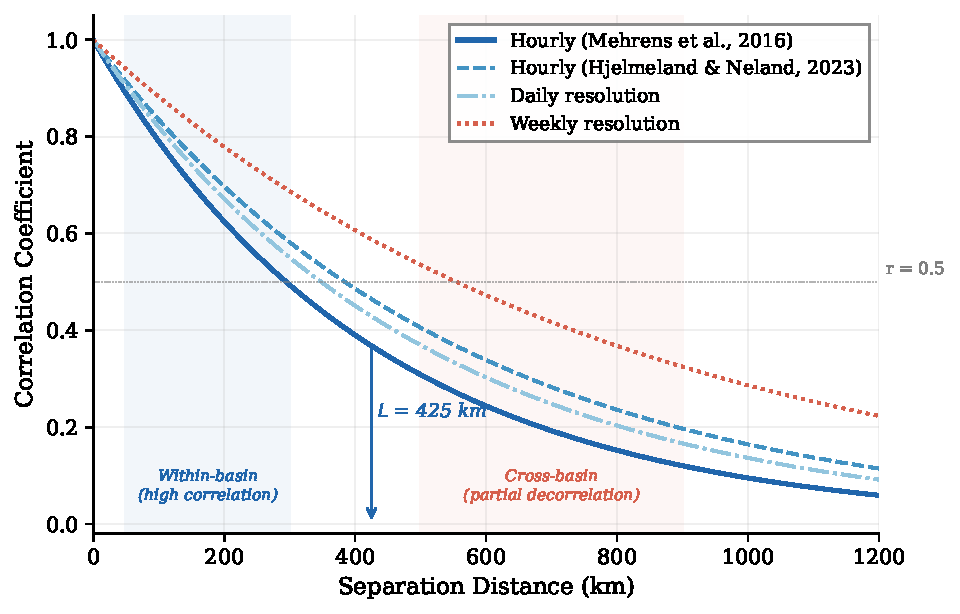
\includegraphics[width=0.72\textwidth]{correlation_decay}
    \caption[Wind power correlation against separation distance]{Wind power correlation against separation distance at different
    temporal resolutions, after Mehrens et al. \cite{Mehrens2016} and
    Hjelmeland and Neland \cite{Hjelmeland2023}. Typical within-basin
    separations (50 to 300~km) sit on the high-correlation shoulder;
    cross-basin separations (500 to 900~km) fall past the decorrelation length
    of about 425~km.}
    \label{fig:correlation_decay}
\end{figure}

Market coupling transmits
price effects across borders, so zones that are physically distant but well
interconnected can show more correlated prices than their wind resources would
suggest. Whether the partial decorrelation of output between the basins survives
into a corresponding decorrelation of capture prices, or whether coupling erodes
that diversification benefit, has not been established, and it bears directly on
whether spreading investment across both basins is a genuine hedge.

\subsubsection{Market structure and the penetration gradient}

The composition of the surrounding fleet sets the slope of the merit order curve
and with it the price response to wind (Figure~\ref{fig:gen_mix}), and four archetypes span the range. Germany, its dispatchable fleet still dominated by
coal, lignite and gas, presents a steep curve in which each increment of wind
produces a large price swing, and its size propagates that volatility to its
neighbours \cite{Ember2025, GermanPrices2023}. Denmark, despite Europe's highest
wind penetration at roughly 55\% of generation, has not seen capture values
collapse as theory predicts, because exceptional interconnection to Nordic hydro
flattens the curve it faces \cite{DanishEnergyAgency2024, Hirth2013}. Sweden,
with hydro near 45\% of production, offers the region's most favourable
environment: at 30\% penetration Hirth estimates wind capture value about
18\% higher in hydro-dominated than thermal-dominated systems \cite{Hirth2013},
wide enough to move a marginal project from loss to viability. Poland sits at
the opposite pole, coal above 60\% of generation \cite{EmberGlobal2024} and
5.9~GW of offshore planned by 2030 \cite{Owczarek2021}, so early projects earn
high capture prices by displacing expensive coal while the programme itself
erodes the conditions that made them attractive. Finland and Estonia are just
entering the same cycle \cite{FinlandOffshoreWind2025, EstoniaOffshoreWind2025}.
Table~\ref{tab:country_archetypes} consolidates the archetypes.

\begin{figure}[!htb]
    \centering
    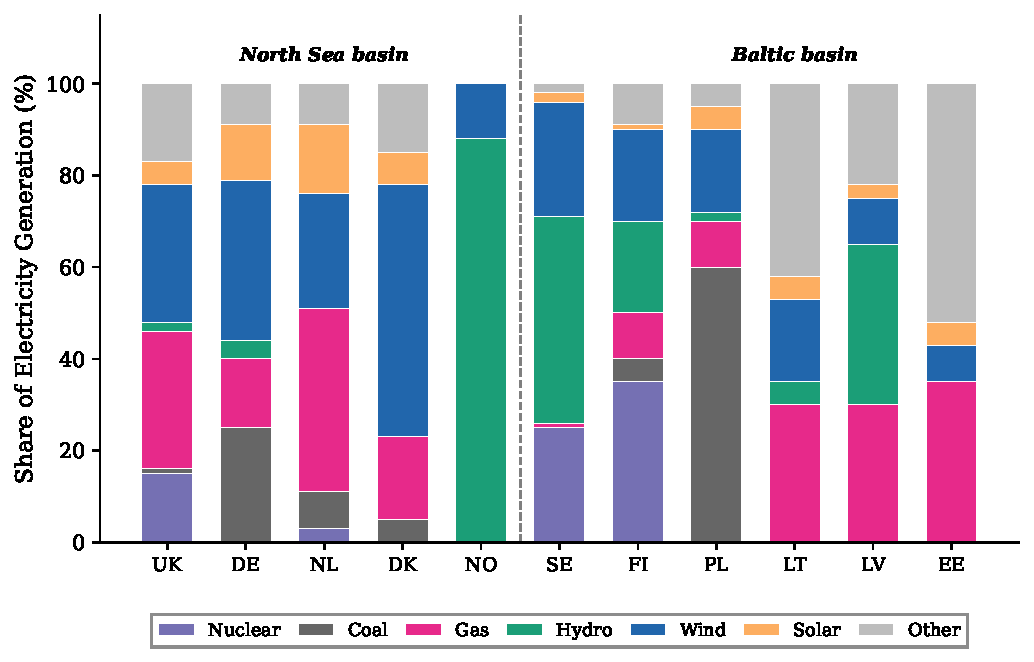
\includegraphics[width=0.9\textwidth]{generation_mix_comparison}
    \caption[Generation mix across the countries bordering the two basins]{Electricity generation mix across the countries bordering the two
    basins, approximate 2024 shares, from Ember \cite{Ember2025} and national
    system operators. Thermal-heavy systems such as Germany and Poland have
    steep merit order curves, in which wind output moves the price sharply.
    Hydro-dominated systems such as Sweden and Norway absorb the same
    variability with little price impact.}
    \label{fig:gen_mix}
\end{figure}

\begin{table}[!htb]
\centering
\small
\caption{Market archetypes around the two basins. Wind penetration and value
factor estimates reflect approximate 2024 values; the final column gives the
dominant revenue support instrument for offshore wind.}
\label{tab:country_archetypes}
\resizebox{\textwidth}{!}{%
\begin{tabular}{l c c l l c c l}
\toprule
\textbf{Country} & \textbf{Basin} & \textbf{Wind (\%)} & \textbf{Dominant gen.} & \textbf{Flexibility} & \textbf{Intercon.} & \textbf{Capture value} & \textbf{Support} \\
\midrule
Germany & NS & $\sim$35 & Gas, coal, wind & Limited; gas peakers & Medium & 0.76--0.85 & Two-sided CfD \\
\addlinespace
Denmark & NS/BS & $\sim$55 & Wind, gas & Nordic hydro (import) & Very high & 0.80--0.90 & CfD (from 2025) \\
\addlinespace
Netherlands & NS & $\sim$25 & Gas, wind & Gas peakers; import & High & 0.85--0.90 & SDE++ tender \\
\addlinespace
UK & NS & $\sim$30 & Gas, wind, nuclear & Gas CCGT; storage & Medium & 0.80--0.85 & CfD (AR rounds) \\
\addlinespace
Sweden & BS & $\sim$25 & Hydro, nuclear, wind & Large hydro reservoirs & High & 0.90--0.95 & Certificates \\
\addlinespace
Finland & BS & $\sim$20 & Nuclear, hydro, wind & Hydro; nuclear baseload & High & 0.90--0.95 & Premium / CfD \\
\addlinespace
Poland & BS & $\sim$18 & Coal, gas & Limited; coal inflexible & Low & 0.95--1.00 & CfD auction \\
\addlinespace
Baltic states & BS & $<$15 & Gas, import, wind & Limited; import-dependent & Medium & $\sim$1.00 & Premium schemes \\
\bottomrule
\end{tabular}%
}
\end{table}

The pattern is striking and, on the conventional reading, paradoxical: every
Baltic market currently records a higher capture value than every North Sea
market, despite uniformly lower interconnection and, in Poland's case, minimal
system flexibility. Penetration is the dominant
predictor of capture value today. Whether that ordering survives as Baltic
capacity scales from single to double-digit gigawatts is the question a
cross-basin comparison exists to answer.

Both basins have committed to expansion on a scale that will settle it: at
least 65~GW of North Sea offshore by 2030 under the Esbjerg Declaration
\cite{Esbjerg2022} and 19.6~GW in the Baltic under Marienborg, a sevenfold
increase \cite{Marienborg2022}, consolidated by ENTSO-E into 146 and 43~GW by
2050 \cite{ONDP2024} against a Baltic technical potential of 93~GW
\cite{Barzehkar2024}. North Sea markets, already at high penetration, face
the steepest marginal declines; Baltic markets begin further back on the
curve. The timing and severity of what follows is a forecasting problem, and
it is to the tools for that problem that the chapter now turns.

\subsection{Models for estimating capture value}\label{sec:modelling}

The question posed in Section~\ref{sec:mitigation}, how much of the value
erosion is removable by design, cannot be answered by any single tool. It
demands four things at once: an hourly generation profile at any point in either
basin, including places where no turbine yet stands; a price for that generation
in the local market, both as it has behaved and as it would behave under a fleet
that does not yet exist; a way to establish that those prices are credible; and a
spatial frame in which locations can be compared on revenue rather than on
energy. Each requirement has its own literature, and each of those literatures stops
short of the others. This section takes them in turn.

\subsubsection{Modelling generation from meteorological data}

A comparison spanning both basins requires one reanalysis product applied
identically to each. Higher-resolution regional products represent coastal
gradients better \cite{Solbrekke2022, Spangehl2021}, but none spans both basins
at the hourly resolution capture value requires. ERA5, at 0.25\textdegree{} and
hourly from 1940, is the only product that does, and it has been validated
against tall towers \cite{Staffell2016, Ramon2019} and North Sea platforms at
$r = 0.85$ to $0.93$ \cite{Bot2024}. Its known weakness is that it
underestimates strong offshore winds, by roughly 15\,\% at 15~m\,s$^{-1}$
\cite{Gandoin2024}, which the cubic relationship between speed and power
amplifies into an error in capacity factor.

Converting wind fields into power follows the standard procedure of Staffell and
Pfenninger \cite{Staffell2016}, now implemented in open tools such as atlite
\cite{Hofmann2021}. A bias correction against fleet data is not optional in that
procedure, since uncorrected reanalysis understates offshore capacity factors by
12 to 15\,\%.

\subsubsection{Models of electricity prices}

Electricity prices are among the hardest commodities to model, combining extreme
volatility, seasonality on several timescales, and mean reversion punctuated by
spikes \cite{Weron2014}. Two of Weron's five families matter here, and the
distinction organises this thesis: statistical models estimate the relationship
between wind and price from what markets have done, and system models rebuild it
from what the system is made of. Behind both sits a general trade-off
\cite{Pfenninger2014, Ringkjob2018}: tools with fine spatial resolution simplify
temporal dynamics, and tools with rich temporal detail aggregate space.
Table~\ref{tab:modelling_comparison} places the principal tools against the
requirements above. Zeyringer et al. \cite{Zeyringer2018} show what the gap
costs: designs that neglect the coincidence of high wind and low prices
overestimate how much capacity is worth building.

\begin{table}[!htb]
\centering
\small
\caption{Principal modelling tools against the requirements of this thesis.
Each covers one dimension of the problem, resource, price, network, or space,
and stops short of the others.}
\label{tab:modelling_comparison}
\resizebox{\textwidth}{!}{%
\begin{tabular}{l l c c p{4.3cm} p{4.3cm}}
\toprule
\textbf{Tool} & \textbf{Type} & \textbf{Spatial} & \textbf{Temporal} &
\textbf{Key strength} & \textbf{Missing dimension} \\
\midrule
atlite \cite{Hofmann2021} & Resource conversion & 0.05--0.25$^{\circ}$ & Hourly &
Open; flexible weather cutouts & No market or revenue component \\
\addlinespace
Renewables.ninja \cite{Staffell2016} & Resource conversion & Site & Hourly &
Bias-corrected; validated globally & No market or revenue component \\
\addlinespace
PyPSA-Eur \cite{Horsch2018} & System optimisation & Nodal & Hourly &
Full European network; open & Shadow prices rather than observed prices \\
\addlinespace
Balmorel \cite{Wiese2018} & System optimisation & Zonal (Nordic--Baltic) & Hourly &
Regional hydro coupling; open & Regional scope; same price caveat \\
\addlinespace
EuroMod \cite{Mendes2024} & Dispatch / market & Zonal (27) & Hourly &
Realistic price volatility & Proprietary data; tied to calibration period \\
\addlinespace
PLEXOS \cite{PLEXOS2024} & Unit commitment & Nodal/zonal & Sub-hourly &
Industry standard; generator detail & Proprietary and costly \\
\addlinespace
Stiewe et al. \cite{Stiewe2025} & Panel regression & Zonal (30+) & Annual &
Cross-border spillovers & Fixed effects absorb the why; no map \\
\addlinespace
Bosch et al. \cite{Bosch2017, Bosch2018, Bosch2019} & GIS spatial & 0.05$^{\circ}$ &
32 slices/yr & Depth, distance, LCOE & No market value or revenue \\
\bottomrule
\end{tabular}%
}
\end{table}

\textbf{Statistical models} estimate the relationship from observed data. Hirth
\cite{Hirth2013} combined meta-regression with dispatch modelling to estimate the
slope of capture value against penetration. Stiewe et al. \cite{Stiewe2025}
extended this to a panel across more than thirty zones,
%
\begin{equation}
    VF_{i,t} = \alpha_i + \beta_1\, WP_{i,t} + \beta_2\,
    \overline{WP}_{N(i),t} + \gamma \mathbf{X}_{i,t} + \varepsilon_{i,t},
    \label{eq:stiewe_model}
\end{equation}
%
where $VF_{i,t}$ is the wind capture value in zone $i$, $WP_{i,t}$ is domestic
wind penetration, $\overline{WP}_{N(i),t}$ is the capacity-weighted penetration
of directly interconnected neighbours, and $\alpha_i$ is a zone fixed effect.
That fixed effect is where the explanatory limit sits: everything that makes one
market different from another is absorbed into a single intercept. Maciejowska
\cite{Maciejowska2020} showed that wind compresses the upper tail of the price
distribution more than it shifts the mean, which is why capture prices fall
faster than average prices, and machine-learning variants have improved
short-term forecasting accuracy over linear specifications
\cite{Lago2021, Marcjasz2023}.

The defining constraint of this family is structural: a model fitted over a
range of conditions describes that range. Tree ensembles, the strongest
performers in recent comparisons \cite{Lago2021}, are piecewise constant by
construction, so beyond the training data no splits exist and the prediction
stops changing. A linear specification will extend beyond its data, but only by
asserting that a slope estimated at penetrations of 10 to 35\,\% still holds at
60\,\%, which is precisely where the evidence says the relationship steepens
\cite{Cevik2022, LopezProl2024}.

\textbf{System models} construct the price instead of fitting it. A
cost-minimising dispatch and investment program returns the shadow price of the
energy balance at each node, which under marginal-cost pricing is the wholesale
price. Green and Vasilakos \cite{GreenVasilakos2011} applied this to the British
market early, finding that large-scale offshore deployment lowers wholesale
prices and with them the revenue of the deployers themselves. PyPSA-Eur
\cite{Horsch2018, PyPSA2024} provides an open implementation with the full
European transmission network at nodal resolution, since extended globally
\cite{PyPSAEarth2024}. Because such a model re-derives the merit order for any
system state, it can price configurations that have never existed, which is what
a 2040 scenario requires.

Its errors are equally structural and run in a known direction. The shadow price
excludes mark-ups, strategic bidding and scarcity rents \cite{Mays2023}. Without
unit commitment the model cannot bid below zero, so it cannot reproduce the
negative prices that are cannibalisation's sharpest symptom \cite{Ruhnau2023}.
Perfect foresight lets storage, and Nordic hydro in particular, absorb surplus at
exactly the right moment. Clustering the network hides congestion inside each
node. Every one of these approximations raises capture value, and each is
largest in small, hydro-adjacent, well-interconnected zones. Commercial tools
relax some of them through non-convex generator constraints
\cite{PLEXOS2024, Mendes2024} but require proprietary plant data, and the Nordic
and Baltic region has its own open lineage in Balmorel \cite{Wiese2018}, which
shares the same approximations. One boundary applies to both families: adding
neighbouring countries' generation and prices measurably reduces day-ahead
forecasting error \cite{VanDerHeijden2021}, so no single-zone model of either
kind sees the whole mechanism.

\subsubsection{Comparison of the two model families}

A statistical model is accurate
where observations are dense, and beyond them it stops responding to its inputs.
A system model can price any future, but it simplifies the market it rebuilds,
and the error that follows is consistently in the same direction. Neither
limitation can be removed by improving a model within its own family.

No study compares them directly: where both estimates of the same quantity
exist, the literature offers no way to decide which to believe, no test for the
point at which one should replace the other, and no comparison with observation
that would reveal the consistent error of the one and the flat response of the
other. Supplying that comparison is one contribution of this thesis.

The tools for making it are standard and have simply not been applied to this
question. They cover the choice of error measure \cite{HyndmanKoehler2006}, the
separation of a consistent offset from other kinds of error \cite{Theil1966},
testing whether a difference in accuracy is real \cite{DieboldMariano1995}, and
holding out whole locations or whole periods rather than individual observations
when data are structured in space and time \cite{Roberts2017}.
Section~\ref{sec:gap_method} sets out how each is used here. What matters for the
argument is that the two families fail differently, so a comparison reporting
only an average error would conceal exactly the difference that decides which
model carries a projection.

\subsubsection{LCOE and its extensions}
\label{sec:vlcoe_lit}

The most developed spatial framework is the progression by Bosch, Staffell
and Hawkes \cite{Bosch2017, Bosch2018, Bosch2019}, which moved from gridded
capacity factors, to offshore depth and distance constraints, to spatially
resolved levelised cost, and was later extended globally \cite{Chu2020}, all
on open bathymetry and resource data \cite{GEBCO2014, GlobalWindAtlas}.
What these frameworks optimise is the levelised cost of energy (LCOE), the
lifetime cost of a project per megawatt-hour produced, which is the standard
basis for comparing technologies and sites \cite{IRENA2025Costs, BCG2025}.

These frameworks characterise cost comprehensively and revenue not at all. A
site with low levelised cost may still return poorly if it sells into a market
where cannibalisation has driven capture prices below that cost.

A parallel literature has long argued that levelised cost is the wrong
comparator. Ueckerdt et al. \cite{Ueckerdt2013} decomposed integration cost into
profile, balancing and grid components, of which profile cost is exactly the
capture value shortfall of Section~\ref{sec:value_problem}; Hirth
\cite{Hirth2015} made the same argument through market value; the International
Energy Agency operationalised it as the value-adjusted levelised cost of
electricity \cite{IEAValcoe2018}; and Joskow \cite{Joskow2019} had earlier
objected that comparing levelised costs across technologies with different
output profiles is economically meaningless.

The gap is that the two literatures have been kept apart. Value-adjusted metrics
are computed for a technology within a system; spatial frameworks for a location
within a map. Nobody has computed a value-adjusted cost \textit{per location},
which is what an investor choosing between a Polish and a German site needs, and
which is necessary before asking whether a ranking of sites by cost survives the
addition of value.

This thesis closes that gap with one derived metric. A merchant farm breaks
even when the price it captures covers its levelised cost; its captured price
is $\bar p\,\mathrm{CV}$ (Equation~\ref{eq:value_factor}), so the average
wholesale price a site needs is
%
\begin{equation}
  \mathrm{vLCOE} \;=\; \frac{\mathrm{LCOE}}{\mathrm{CV}},
  \label{eq:vlcoe}
\end{equation}
%
the \emph{value-adjusted LCOE}. Where the IEA's VALCOE adjusts a technology's
cost additively within one system \cite{IEAValcoe2018}, this metric is
multiplicative, carries the measured capture value directly, and is computed per
location, so it can be mapped. Because capture value sits in the denominator it
can rise even as the raw LCOE falls, whenever cannibalisation erodes value
faster than learning cuts cost.

\subsection{Research gaps and questions}\label{sec:research_gap}

Four gaps follow from the review.

\textbf{No systematic cross-basin comparison of capture value.} Capture values
have been measured within national markets and across a European panel
\cite{Stiewe2025}, but no study compares them across the full set of bidding
zones surrounding both basins under a consistent method, and merit order
estimates for Baltic markets are effectively absent \cite{Cevik2022}.

\textbf{Cannibalisation is treated as a property of penetration rather than of
system design.} The decline is well documented and interconnection and
flexibility are known to moderate it
\cite{Stiewe2025, Schlachtberger2017, OffshoreHybrids2024}, but the literature
does not decompose a decline into the portion a different system configuration
would remove and the portion that is structural. Without that split, a capture
value figure cannot distinguish a transmission problem from an oversupply
problem, and the policy implications of the two are opposite.

\textbf{Market value is absent from spatial assessment, and support design from
both.} GIS frameworks rank sites on cost while ignoring revenue
\cite{Bosch2017, Bosch2018, Bosch2019}, and the contract-design literature
\cite{Beiter2024, Kitzing2024, Dukan2025, Anatolitis2025} treats revenue risk as
a financing question rather than asking which physical component of a value
decline a given instrument absorbs.

\textbf{No method both measures and projects.} Statistical models are accurate
in sample and cannot extrapolate beyond their support; system models project
freely and carry structural bias. The literature offers no validated procedure
for combining them or for establishing at which point one should replace the other.

These gaps motivate three research questions.

\begin{enumerate}
    \item How does offshore wind capture value in the enclosed Baltic compare
    with the open North Sea today, and how does it evolve under the committed
    buildout to 2030 and 2040?
    \item Which market mechanisms determine the rate of value erosion, do they
    differ between an enclosed and an open basin, and how much of the erosion is
    removable by system design rather than inherent to the resource?
    \item Can a model trained on historical observation project these futures, or
    is a system model required, and how should the two be combined and validated
    against each other?
\end{enumerate}

The third question is the one on which the other two depend, since every
projected number in this thesis comes from one model or the other, and it is the
one the literature leaves most open. This thesis builds one model of
each kind, a statistical model fitted to eight years of observed prices and a
system model that rebuilds the market from physics and cost, and sets them side
by side. Somewhere the two will disagree, and the practical decision is which of
them produces the 2040 numbers this thesis reports. Section~\ref{sec:confrontation}
sets out how that decision is made from measurement rather than by inspection.

Answering the first question is of limited use if the answer stops at a ratio.
A capture value only changes a decision once it is priced, so this thesis also
carries the projected values onto the map and folds them into cost, giving the
average wholesale price each location must earn to break even. That step turns
the measured erosion into the question an investor faces, which is
where to build and whether the cheapest site is still the best one.

Answering these requires four objectives, running from the apparatus outward to
the decisions it informs.

\begin{enumerate}
    \item \textit{Build and validate the two models.} Construct a virtual wind
    farm from reanalysis and validate it against metered generation; fit a
    capture value model carrying market characteristics as explicit features
    rather than fixed effects, scored by leaving whole farms out; configure an
    open system model of both basins under official capacity trajectories; and
    confront both against observation where reality can arbitrate.

    \item \textit{Measure and project capture value across both basins.}
    Establish where each bidding zone stands today and how it evolves to 2030
    and 2040 under the committed buildout.

    \item \textit{Decompose the erosion into removable and structural parts.}
    Separate what an unconstrained network or a flexible demand side would
    remove from what the buildout imposes regardless, and identify who bears
    each part once support contracts are accounted for.

    \item \textit{Map the value-adjusted cost of energy and test whether capture value
    changes where to build.} Carry the validated capture values onto the map
    alongside resource, water depth and distance to shore, and fold them into
    cost to give a \textit{value-adjusted levelised cost of energy}, the average
    wholesale price a site must earn to break even, computed per location rather
    than per technology. Then compare the ranking of candidate sites by cost
    alone against the ranking once value is included. If the rankings agree a
    cost-only screen is sufficient; if they diverge, site selection has been
    made on an incomplete criterion, and the divergence grows over the period
    across which projects are financed.

    \end{enumerate}

The remainder of this thesis pursues these objectives using open data
throughout, so that every step from raw download to final figure can be
inspected and re-run.
